\documentclass[12pt]{article}

\usepackage[utf8x]{inputenc} % Включаем поддержку UTF8  
\usepackage[russian]{babel}  % Включаем пакет для поддержки русского языка  
\usepackage{hyperref}        % Для гиперссылок

% Математика
\usepackage{amsmath}         % В т.ч. для матриц
\usepackage{amssymb}

% Прога
\usepackage{etoolbox}
\usepackage{listings}

% Цвета
\usepackage{xcolor}

% Картинки
\usepackage{graphicx}
\graphicspath{ {./images/} }

\newtheorem{property}{Свойство}
\newtheorem{consequence}{Следствие}[property]

\newcommand{\qedsymbol}{\rule{2mm}{2mm}}

\begin{document}

\thispagestyle{empty}
\begin{center}
\textbf{ПРАВИТЕЛЬСТВО РОССИЙСКОЙ ФЕДЕРАЦИИ}

\vspace{5ex}
	
\textbf{Федеральное государственное автономное образовательное учреждение \\ высшего образования \\ <<Национальный исследовательский университет \\ <<Высшая школа экономики>>}
\end{center}
\vspace{5ex}

\begin{center}
    Московский институт электроники и математики им. А.Н. Тихонова  
    
    \vspace{5ex}
    
    Департамент прикладной математики
    
    \vspace{10ex}
    \textbf{Отчёт \\ по лабораторной работе №3 \\ по курсу <<Алгоритмизация и программирование>>}
	\vspace{7ex}

\end{center}

\begin{center} 
\begin{tabular}{| p{0.3\linewidth}| p{0.3\linewidth}| p{0.3\linewidth}|}
 \hline	
ФИО студента & Номер группы & Дата \\  \hline
 & & \\  
Вязов Глеб \newline Дмитриевич & БПМ-231 & 22.10.2023\\  
 & & \\  \hline		
\end{tabular}
\end{center}

\begin{center}
	\vspace{3ex}
	
	\vfill
   
   \normalsize
    
	\textbf{Москва, 2023}
\end{center}

\newpage

%---------------------------------------------------------------------------------

\section*{Задание (вариант №7)}
Вычислить приближенное значение функции, вычислив сумму конечного числа элементов ряда двумя способами, используя разные типы циклов:

\begin{enumerate}
\item с заданной точностью;
\item для заданного количества членов ряда.
\end{enumerate}

Переход к способу вычисления реализовать с помощью оператора выбора.

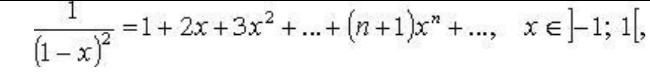
\includegraphics{img1}

\newpage

%---------------------------------------------------------------------------------

\section*{Решение}\addcontentsline{toc}{section}{Решение}

\lstset{ %
texcl=true,%
language=C,                 % выбор языка для подсветки
basicstyle=\small\sffamily, % размер и начертание шрифта для подсветки кода
numbers=left,               % где поставить нумерацию строк (слева\справа)
numberstyle=\tiny,           % размер шрифта для номеров строк
stepnumber=1,                   % размер шага между двумя номерами строк
numbersep=5pt,                % как далеко отстоят номера строк от подсвечиваемого кода
backgroundcolor=\color{white}, % цвет фона подсветки - используем \usepackage{color}
showspaces=false,            % показывать или нет пробелы специальными отступами
showstringspaces=false,      % показывать или нет пробелы в строках
showtabs=false,             % показывать или нет табуляцию в строках
frame=single,              % рисовать рамку вокруг кода
tabsize=3,                 % размер табуляции по умолчанию равен 2 пробелам
captionpos=t,              % позиция заголовка вверху [t] или внизу [b] 
breaklines=true,           % автоматически переносить строки (да\нет)
breakatwhitespace=false, % переносить строки только если есть пробел
escapeinside={\%*}{*)},   % если нужно добавить комментарии в коде
inputencoding=utf8x,
extendedchars=\true
}

\begin{lstlisting}[label=string_code1,caption=C]
#include <stdio.h>
#include <math.h>

// Функция считает сумму конечного числа для заданного количества членов ряда
double a_n_with_epsilon(double x) {
    double e;
    printf("\nВведите точность: ");
    scanf("%lf", &e);

    double a_n = 1;
    double summa = a_n;
    int i = 1;
    
    // Цикл работает пока модуль элемента будет больше e
    // Как только мы достигнет заданной точности, цикл прервется
    while (fabs(a_n) > e) {
        a_n = a_n * x * (i+1) / i;
        summa += a_n;
        i++;
    }

    return summa;
}

// Функция считает сумму конечного числа с заданной точностью
double a_n_with_n(double x) {
    int n;
    printf("\nВведите количество членов ряда: ");
    scanf("%d", &n);

    double a_n = 1;
    double summa = a_n;
    
    // Цикл делает n-1 операцию
    // Первая операция уже сделана
    for (int i=1; i<n; i++) {
        a_n = a_n * x * (i+1) / i;
        summa += a_n;
    }

    return summa;
}

int main() {
    // Меняем кодировку на UTF-8, чтобы можно было писать на русском
    system("chcp 65001");

    int flag;
    double x;

    // Ввод переменных. Дружественный интерфейс
    printf("Выполнил задание: Вязов Глеб. Группа: БПМ231\n");
    printf("Введите x = ");
    scanf("%lf", &x);

    // Проверка x на корректность
    if (!(-1 < x && x < 1)) {
        printf("x не принадлежит промежутку (-1; 1)");
        return 0;
    }

    printf("По формуле = %lf", 1.0 / ((1-x)*(1-x)));

    // Ввод переменных. Дружественный интерфейс
    printf("\nВведите 1, если Вы хотите использовать цикл с заданной точностью");
    printf("\nВведите 2, если Вы хотите использовать цикл для заданного количества членов ряда: ");
    scanf("%d", &flag);
    
    // Оператор выбора swith-case-default
    switch (flag) {
        case 1: printf("%lf", a_n_with_epsilon(x)); break;
        case 2: printf("%lf", a_n_with_n(x)); break;
        default: printf("\nЯ не знаю такой команды :(");
    }

    return 0;
}
\end{lstlisting} 

\newpage

%---------------------------------------------------------------------------------

\section*{Тестирование}

\begin{enumerate}

\item \textbf{Тест №1.} 

\textit{Ввод:} 0.5, 1, 0.001

\textit{Вывод:} 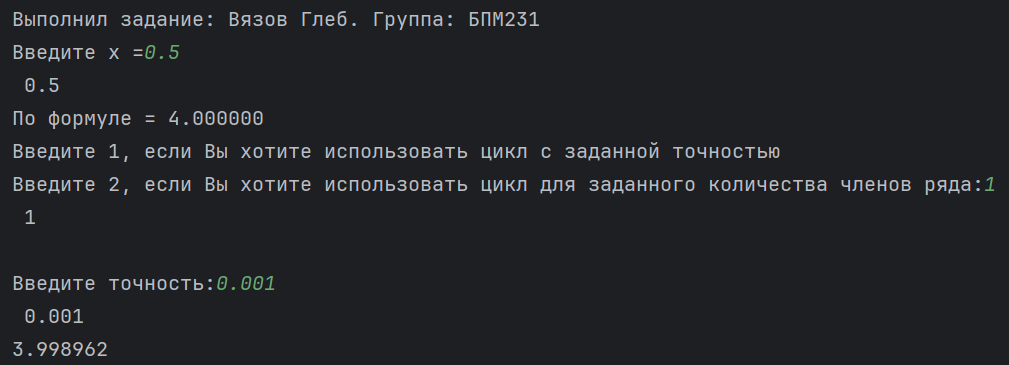
\includegraphics[width=0.9\textwidth]{img2}



\item \textbf{Тест №2.}

\textit{Ввод:} 0.5, 2, 10

\textit{Вывод:} 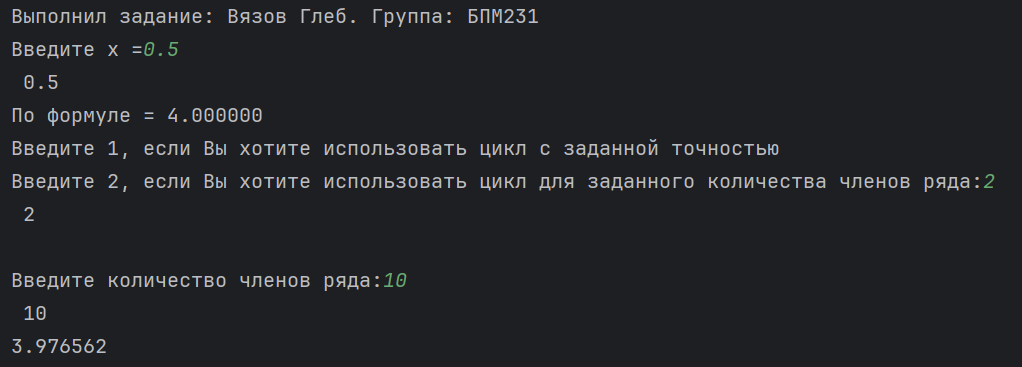
\includegraphics[width=0.9\textwidth]{img3}



\item \textbf{Тест №3.}

\textit{Ввод:} 0.5, 3

\textit{Вывод:} 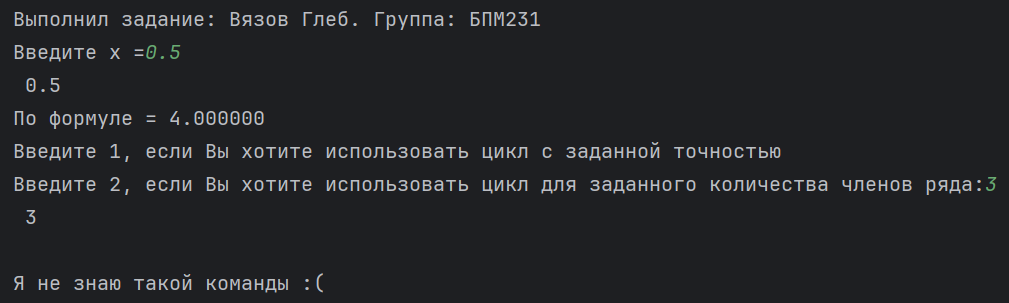
\includegraphics[width=0.9\textwidth]{img4}



\end{enumerate}


\end{document}
